% Created 2024-12-02 lun 12:39
% Intended LaTeX compiler: pdflatex
\documentclass[10pt]{article}
\usepackage[utf8]{inputenc}
\usepackage{lmodern}
\usepackage[T1]{fontenc}
\usepackage[top=1in, bottom=1.in, left=1in, right=1in]{geometry}
\usepackage{graphicx}
\usepackage{longtable}
\usepackage{float}
\usepackage{wrapfig}
\usepackage{rotating}
\usepackage[normalem]{ulem}
\usepackage{amsmath}
\usepackage{textcomp}
\usepackage{marvosym}
\usepackage{wasysym}
\usepackage{amssymb}
\usepackage{amsmath}
\usepackage[theorems, skins]{tcolorbox}
\usepackage[version=3]{mhchem}
\usepackage[numbers,super,sort&compress]{natbib}
\usepackage{natmove}
\usepackage{url}
\usepackage[cache=false]{minted}
\usepackage[strings]{underscore}
\usepackage[linktocpage,pdfstartview=FitH,colorlinks,
linkcolor=blue,anchorcolor=blue,
citecolor=blue,filecolor=blue,menucolor=blue,urlcolor=blue]{hyperref}
\usepackage{attachfile}
\usepackage{setspace}
\usepackage[spanish, ]{babel}
\date{}
\title{Índice de precios de viviendas nuevas y de segunda mano}
\begin{document}

\maketitle
\section*{Los datos}
\label{sec:org7cea968}

Los datos de este ejercicio corresponden a los índices de precios de
vivienda nueva y de segunda mano con base 2015. La muestra disponible
incluye 64 observaciones trimestrales, comprendidas entre el primer
trimestre de 2007 y el cuarto de 2022. \textbf{Fuente:} Instituto Nacional de
Estadística.
\begin{minted}[frame=lines,fontsize=\scriptsize,linenos=]{r}
open IndicePreciosViviendasNuevasYdeSegundaMano.gdt
\end{minted}
\begin{description}
\item[{\texttt{IPVN}}] Índice de precios de vivienda nueva, base 2015.
\item[{\texttt{IPV2M}}] Índice de precios de vivienda de segunda mano, base 2015.
\end{description}
A partir de esta muestra, se calculan las tasas de variación anual:
\begin{center}
\begin{tabular}{ll}
\(T4IPVN_t=100\times\left(\frac{IPVN_t}{IPVN_{t-1}}-1\right);\quad\) & \(T4IPV2M_t=100\times\left(\frac{IPV2M_t}{IPV2M_{t-1}}-1\right)\).\\
\end{tabular}
\end{center}
\begin{description}
\item[{\texttt{T4IPVN}}] Tasa de variación anual de \texttt{IPVN}.
\item[{\texttt{T4IPV2M}}] Tasa de variación anual de \texttt{IPV2M}.
\end{description}

Ficheros \url{https://github.com/mbujosab/EconometriaAplicada-SRC/tree/main/Ejercicios}
\begin{itemize}
\item Versión en \href{https://github.com/mbujosab/EconometriaAplicada-SRC/blob/main/Ejercicios/IndicePreciosViviendasNuevasYdeSegundaMano.pdf}{pdf}
\item Datos: \href{IndicePreciosViviendasNuevasYdeSegundaMano.gdt}{IndicePreciosViviendasNuevasYdeSegundaMano.gdt}
\item Guión de gretl: \href{IndicePreciosViviendasNuevasYdeSegundaMano.inp}{IndicePreciosViviendasNuevasYdeSegundaMano.inp}
\end{itemize}
\section*{Gráfico de las tasas de variación los índices de precios}
\label{sec:org1f47220}

\begin{minted}[frame=lines,fontsize=\scriptsize,linenos=]{r}
gnuplot T4IPVN T4IPV2M  --time-series --with-lines --output="TasasDeVariacionAnual.png"
\end{minted}

\phantomsection
\label{GráficoTasasVariación}
\begin{center}
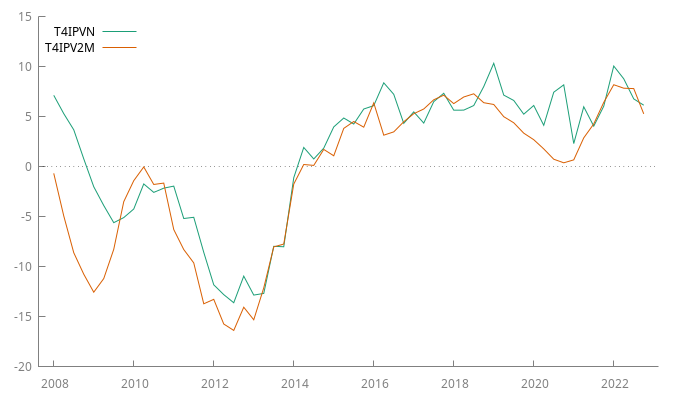
\includegraphics[width=0.5\textwidth]{./IndicePreciosViviendasNuevasYdeSegundaMano/TasasDeVariacionAnual.png}
\end{center}

El perfil de las series que se muestran en la \hyperref[sec:org1f47220]{figura anterior} sugiere que
ambas podrían estar cointegradas. Para estudiar esta posibilidad se
estiman:
\begin{itemize}
\item \hyperref[sec:org8c8f2d8]{modelos ARIMA} para las series \texttt{T4IPVN} y \texttt{T4IPV2M}, así como
\item \hyperref[sec:org380d85c]{un modelo AR(1) para la serie \texttt{T4IPVN} con \texttt{T4IPV2M} y como input
exógeno}.
\end{itemize}
\section*{Modelos ARIMA}
\label{sec:org8c8f2d8}

\subsection*{Vivienda nueva}
\label{sec:org12fdb89}

Se ajusta el siguiente modelo estacional para  \texttt{T4IPVN}:
\begin{minted}[frame=lines,fontsize=\scriptsize,linenos=]{r}
ARIMA_T4IPVN <- arima 0 1 0 ; 0 0 1 ; T4IPVN --nc
modtest --normality --quiet
modtest --arch --quiet
modtest --autocorr 15 --quiet
\end{minted}

\begin{verbatim}
Evaluaciones de la función: 16
Evaluaciones del gradiente: 9

ARIMA_T4IPVN:
ARIMA, usando las observaciones 2008:2-2022:4 (T = 59)
Estimado usando AS 197 (MV exacta)
Variable dependiente: (1-L) T4IPVN
Desviaciones típicas basadas en el Hessiano

             coeficiente   Desv. típica     z      valor p
  --------------------------------------------------------
  Theta_1     −0,352053      0,161467     −2,180   0,0292  **

Media de la vble. dep. −0,016781   D.T. de la vble. dep.   2,324958
Media de innovaciones  −0,003088   D.T. innovaciones       2,208917
R-cuadrado              0,889602   R-cuadrado corregido    0,889602
Log-verosimilitud      −130,7397   Criterio de Akaike      265,4793
Criterio de Schwarz     269,6344   Crit. de Hannan-Quinn   267,1013

                       Real Imaginaria     Módulo Frecuencia
  -----------------------------------------------------------
  MA (estacional)
   Raíz  1           2,8405     0,0000     2,8405     0,0000
  -----------------------------------------------------------

ARIMA_T4IPVN guardado

Contraste de la hipótesis nula de distribución Normal:
Chi-cuadrado(2) = 0,287 con valor p 0,86644


Contraste de ARCH de orden 4

Estadístico de contraste: TR^2 = 2,096460,
con valor p = P(Chi-cuadrado(4) > 2,096460) = 0,718023


Contraste de autocorrelación hasta el orden 15

Ljung-Box Q' = 12,8016,
con valor p = P(Chi-cuadrado(14) > 12,8016) = 0,5422
\end{verbatim}
\subsection*{Vivienda de segunda mano}
\label{sec:org440e803}

Se ajusta el siguiente modelo estacional para \texttt{T4IPV2M}:
\begin{minted}[frame=lines,fontsize=\scriptsize,linenos=]{r}
ARIMA_T4IPV2M <- arima 2 1 0 ; 0 0 1 ; T4IPV2M --nc
modtest --normality --quiet
modtest --arch --quiet
modtest --autocorr 15 --quiet
\end{minted}

\begin{verbatim}
Evaluaciones de la función: 37
Evaluaciones del gradiente: 14

ARIMA_T4IPV2M:
ARIMA, usando las observaciones 2008:2-2022:4 (T = 59)
Estimado usando AS 197 (MV exacta)
Variable dependiente: (1-L) T4IPV2M
Desviaciones típicas basadas en el Hessiano

             coeficiente   Desv. típica     z      valor p 
  ---------------------------------------------------------
  phi_1        0,290799      0,118903      2,446   0,0145   **
  phi_2        0,510969      0,149725      3,413   0,0006   ***
  Theta_1     −0,843988      0,177320     −4,760   1,94e-06 ***

Media de la vble. dep.  0,100821   D.T. de la vble. dep.   2,138823
Media de innovaciones   0,069384   D.T. innovaciones       1,521217
R-cuadrado              0,957548   R-cuadrado corregido    0,956032
Log-verosimilitud      −110,6874   Criterio de Akaike      229,3748
Criterio de Schwarz     237,6849   Crit. de Hannan-Quinn   232,6187

                       Real Imaginaria     Módulo Frecuencia
  -----------------------------------------------------------
  AR
   Raíz  1           1,1430     0,0000     1,1430     0,0000
   Raíz  2          -1,7122     0,0000     1,7122     0,5000
  MA (estacional)
   Raíz  1           1,1849     0,0000     1,1849     0,0000
  -----------------------------------------------------------

ARIMA_T4IPV2M guardado

Contraste de la hipótesis nula de distribución Normal:
Chi-cuadrado(2) = 1,017 con valor p 0,60142


Contraste de ARCH de orden 4

Estadístico de contraste: TR^2 = 0,710542,
con valor p = P(Chi-cuadrado(4) > 0,710542) = 0,950023


Contraste de autocorrelación hasta el orden 15

Ljung-Box Q' = 19,2946,
con valor p = P(Chi-cuadrado(12) > 19,2946) = 0,08166
\end{verbatim}
\section*{Modelo ARMAX}
\label{sec:org380d85c}

Se ajusta el siguiente modelo autorregresivo para \texttt{T4IPVN}, con una
constante y \texttt{T4IPV2M} como variables exógenas:

\begin{minted}[frame=lines,fontsize=\scriptsize,linenos=]{r}
ARMAX_T4IPVN <- arima 1 0 0 ; T4IPVN T4IPV2M 0
modtest --normality --quiet
modtest --arch --quiet
modtest --autocorr 15 --quiet
\end{minted}

\begin{verbatim}
Evaluaciones de la función: 18
Evaluaciones del gradiente: 8

ARMAX_T4IPVN:
ARMAX, usando las observaciones 2008:1-2022:4 (T = 60)
Estimado usando AS 197 (MV exacta)
Variable dependiente: T4IPVN
Desviaciones típicas basadas en el Hessiano

             coeficiente   Desv. típica     z     valor p 
  --------------------------------------------------------
  const       2,36047       1,32670       1,779   0,0752   *
  phi_1       0,821915      0,0858539     9,573   1,03e-21 ***
  T4IPV2M     0,612342      0,126633      4,836   1,33e-06 ***

Media de la vble. dep.  1,368477   D.T. de la vble. dep.   6,683657
Media de innovaciones  −0,108356   D.T. innovaciones       1,943328
R-cuadrado              0,917639   R-cuadrado corregido    0,916219
Log-verosimilitud      −125,5632   Criterio de Akaike      259,1265
Criterio de Schwarz     267,5038   Crit. de Hannan-Quinn   262,4033

                       Real Imaginaria     Módulo Frecuencia
  -----------------------------------------------------------
  AR
   Raíz  1           1,2167     0,0000     1,2167     0,0000
  -----------------------------------------------------------

ARMAX_T4IPVN guardado

Contraste de la hipótesis nula de distribución Normal:
Chi-cuadrado(2) = 0,050 con valor p 0,97554


Contraste de ARCH de orden 4

Estadístico de contraste: TR^2 = 5,586830,
con valor p = P(Chi-cuadrado(4) > 5,586830) = 0,232202


Contraste de autocorrelación hasta el orden 15

Ljung-Box Q' = 9,64319,
con valor p = P(Chi-cuadrado(14) > 9,64319) = 0,7878
\end{verbatim}
\subsection*{Intervalo de confianza de los parámetros estimados}
\label{sec:org2d000d3}

Los intervalos de confianza al 95 para los coeficientes del modelo
anterior se muestra a continuación.

\begin{verbatim}
z(0,025) = 1,9600

      VARIABLE         COEFICIENTE      INTERVALO DE CONFIANZA 95%

         const            2,36047        -0,239821      4,96075
         phi_1            0,821915        0,653645     0,990186
       T4IPV2M            0,612342        0,364146     0,860538
\end{verbatim}
\section*{Preguntas}
\label{sec:orgc784893}

\subsection*{Pregunta 1}
\label{sec:org01e80a1}

Comente exhaustivamente los resultados de estimación y diagnosis de
los \hyperref[sec:org8c8f2d8]{modelos ARIMA} estimados. 

(\hyperref[sec:org62462b1]{Respuesta 1})
\subsection*{Pregunta 2}
\label{sec:org6564113}

Compare de todas las formas posibles los modelos \hyperref[sec:org8c8f2d8]{ARIMA} y \hyperref[sec:org380d85c]{ARMAX} de la
variable \texttt{T4IPVN}. ¿Cuál de los dos modelos
\begin{itemize}
\item ajusta mejor la muestra?
\item cabe esperar que produzca mejores previsiones extra-muestrales?
(suponiendo que se conoce el valor de la variable explicativa en el
caso del modelo \hyperref[sec:org380d85c]{ARMAX})
\item cabe esperar que esté mejor especificado?
\end{itemize}

Argumente su respuesta de todas las formas posibles.

(\hyperref[sec:org9943c3f]{Respuesta 2})
\subsection*{Pregunta 3}
\label{sec:org157de2f}

\begin{enumerate}
\item Suponga que los modelos \hyperref[sec:org8c8f2d8]{ARIMA} (para \texttt{T4IPVN} y \texttt{T4IPV2M}) y \hyperref[sec:org380d85c]{ARMAX}
(para \texttt{T4IPVN}) están correctamente identificados y
estimados. Considerando las estimaciones puntuales que se muestran,
discuta detalladamente si las series \texttt{T4IPVN} y \texttt{T4IPV2M} están
cointegradas (en este caso indique cuál es el vector de
cointegración) o si, por el contrario, no lo están.

\item Los \hyperref[sec:org2d000d3]{intervalos de confianza de los parámetros estimados} ¿Introducen
algún matiz en su respuesta previa? ¿O no la afectan en absoluto?
\end{enumerate}

(\hyperref[sec:orgab01ed3]{Respuesta 3})
\subsection*{Pregunta 4}
\label{sec:org496260e}

Indique cuáles de las siguientes expresiones representan el modelo \hyperref[sec:org8c8f2d8]{ARIMA} ajustado a \texttt{T4IPV2M} con un redondeo a tres decimales.

Indique cuáles de las siguientes expresiones NO están bien definidas.


\begin{description}
\item[{Expresión 1}] \(\nabla x_t = \frac{1-0.844 \, \mathsf{B}^4}{1 - 0.291 \mathsf{B} -0.511 \mathsf{B}^2} \hat{a}_t\)
\item[{Expresión 2}] \(\nabla x_t = \frac{1-0.844 \, \mathsf{B}^4}{1 + 0.291 \mathsf{B} +0.511 \mathsf{B}^2} \hat{a}_t\)
\item[{Expresión 3}] \(\nabla x_t = \frac{1+0.844 \, \mathsf{B}^4}{1 - 0.291 \mathsf{B} -0.511 \mathsf{B}^2} \hat{a}_t\)
\item[{Expresión 4}] \(x_t = \frac{1+0.844 \, \mathsf{B}^4}{\nabla(1 + 0.291 \mathsf{B} +0.511 \mathsf{B}^2)} \hat{a}_t\)
\item[{Expresión 5}] \(x_t = \frac{1-0.844 \, \mathsf{B}^4}{\nabla(1 + 0.291 \mathsf{B} +0.511 \mathsf{B}^2)} \hat{a}_t\)
\item[{Expresión 6}] \(x_t-X_{t-1} = \frac{1-0.844 \, \mathsf{B}^4}{1 - 0.291 \mathsf{B} -0.511 \mathsf{B}^2} \hat{a}_t\)
\item[{Expresión 7}] \(x_t-X_{t-1} = \frac{1-0.844 \, \mathsf{B}^4}{1 + 0.291 \mathsf{B} +0.511 \mathsf{B}^2} \hat{a}_t\)
\item[{Expresión 8}] \(x_t+X_{t-1} = \frac{1+0.844 \, \mathsf{B}^4}{1 - 0.291 \mathsf{B} -0.511 \mathsf{B}^2} \hat{a}_t\)
\item[{Expresión 9}] \(\nabla (1 - 0.291 \mathsf{B} - 0.511 \mathsf{B}^2) x_t = (1 - 0.844 \mathsf{B}^4) \hat{a}_t\)
\item[{Expresión 10}] \(\nabla (1 + 0.291 \mathsf{B} + 0.511 \mathsf{B}^2) x_t = (1 - 0.844 \mathsf{B}^4) \hat{a}_t\)
\item[{Expresión 11}] \(\nabla (1 - 0.291 \mathsf{B} - 0.511 \mathsf{B}^2) x_t = (1 + 0.844 \mathsf{B}^4) \hat{a}_t\)
\item[{Expresión 12}] \(\frac{1 -0.291 \mathsf{B} - 0.511 \mathsf{B}^2}{1 - 0.844 \mathsf{B}^4}\nabla x_t = \hat{a}_t\)
\item[{Expresión 13}] \(\frac{1}{1 - 0.844 \mathsf{B}^4}\nabla x_t = \frac{1}{1 -0.291 \mathsf{B} - 0.511 \mathsf{B}^2} \hat{a}_t\)
\item[{Expresión 14}] \(\frac{1}{1 + 0.844 \mathsf{B}^4} x_t = \frac{1}{\nabla(1 -0.291 \mathsf{B} - 0.511 \mathsf{B}^2)} \hat{a}_t\)
\item[{Expresión 15}] \(\frac{1}{1 - 0.844 \mathsf{B}^4} x_t = \frac{1}{\nabla(1 +0.291 \mathsf{B} + 0.511 \mathsf{B}^2)} \hat{a}_t\)

(\hyperref[sec:orge3c0c37]{Respuesta 4})
\end{description}
\subsection*{Pregunta 5}
\label{sec:org55d1589}

Indique cuáles de las siguientes expresiones representan el modelo \hyperref[sec:org380d85c]{ARMAX} ajustado a \texttt{T4IPVN} con un redondeo a tres decimales.

\begin{description}
\item[{Expresión 1}] \(T4IPVN_t = 2.361 + 0.612 \, (T4IPV2M_t) + \frac{1}{1 + 0.822 \mathsf{B}} \hat{a}_t\)
\item[{Expresión 2}] \(T4IPVN_t = 2.361 + 0.612 \, (T4IPV2M_t) + \frac{1}{1 - 0.822 \mathsf{B}} \hat{a}_t\)
\item[{Expresión 3}] \((1 - 0.822 \mathsf{B}) T4IPVN_t = 2.361 + 0.612 \, (T4IPV2M_t) + \hat{a}_t\)
\item[{Expresión 4}] \((1 - 0.822 \mathsf{B}) (T4IPVN_t - 2.361) =  0.612 \, (T4IPV2M_t) + \hat{a}_t\)
\item[{Expresión 5}] \((1 - 0.822 \mathsf{B}) \big(T4IPVN_t - 0.612 \, (T4IPV2M_t) - 2.361\big) = \hat{a}_t\)
\end{description}

(\hyperref[sec:org9955fbd]{Respuesta 5})
\subsection*{Pregunta 6}
\label{sec:org3bf30e1}

Indique si es cierta o no la siguiente afirmación:
\begin{quote}
El criterio de Akaike del modelo \hyperref[sec:org8c8f2d8]{ARIMA} ajustado a \texttt{T4IPV2M} es menor
que el del modelo \hyperref[sec:org8c8f2d8]{ARIMA} ajustado a \texttt{T4IPVN}, lo que indica que el
primer modelo probablemente predecirá fuera de la muestra mejor que el
segundo.
\end{quote}

(\hyperref[sec:orgabe2af9]{Respuesta 6})
\subsection*{Pregunta 7}
\label{sec:orga8641da}

Indique si es cierta o no la siguiente afirmación:

\begin{quote}
La pendiente estimada de la variable \texttt{T4IPV2M} en el modelo \hyperref[sec:org380d85c]{ARMAX}
indica que, si aumenta en un \texttt{1\%} la tasa anual de variación del
índice de precios de la vivienda de segunda mano \texttt{T4IPV2M}, cabe
esperar que la tasa de variación del índice de precios de la vivienda
nueva \texttt{T4IPVN\_t} aumente en un \texttt{0.612\%}.
\end{quote}

(\hyperref[sec:orgc963a3c]{Respuesta 7})
\subsection*{Pregunta 8}
\label{sec:org1ae4693}

Indique si es cierta o no la siguiente afirmación:

\begin{quote}
La pendiente estimada de la variable \texttt{T4IPV2M} en el modelo \hyperref[sec:org380d85c]{ARMAX}
indica que, si aumenta en un punto porcentual la tasa anual de
variación del índice de precios de la vivienda de segunda mano
\texttt{T4IPV2M}, cabe esperar que la tasa de variación del índice de precios
de la vivienda nueva \texttt{T4IPVN} aumente en \texttt{0.612} puntos.
\end{quote}

(\hyperref[sec:org919af4b]{Respuesta 8})
\subsection*{Pregunta 9}
\label{sec:org48a22b3}

Indique si es cierta o no la siguiente afirmación:

\begin{quote}
Los resultados que se muestran en la tabla de \hyperref[sec:org2d000d3]{intervalos de confianza}
indican que debe rechazarse la hipótesis nula de que el parámetro
\(\phi_1\) sea igual a 1 con un 10\% de significación.
\end{quote}

(\hyperref[sec:org5f65151]{Respuesta 9})
\subsection*{Pregunta 10}
\label{sec:orgca7a355}

Indique si es cierta o no la siguiente afirmación:

\begin{quote}
Los resultados que se muestran en la tabla de \hyperref[sec:org2d000d3]{intervalos de confianza}
sugieren que probablemente no se rechazaría la hipótesis nula de que
el parámetro \(phi_1\) sea igual a 1 con un 1\% de significación.
\end{quote}

(\hyperref[sec:org9e54142]{Respuesta 10})
\section*{Respuestas}
\label{sec:orgadc58cd}

\subsection*{Respuesta 1}
\label{sec:org62462b1}

En ambos modelos

\begin{itemize}
\item todos los coeficientes estimados son significativos a los niveles de
confianza habituales, y

\item los contrastes residuales no rechazan a los niveles de confianza habituales las hipótesis nulas de 
\begin{enumerate}
\item normalidad,
\item homoscedasticidad (ausencia de efectos ARCH) y
\item ausencia de autocorrelación.
\end{enumerate}

\item En ambos casos son modelos ARIMA no estacionarios.
\end{itemize}

(\hyperref[sec:org01e80a1]{Pregunta 1})
\subsection*{Respuesta 2}
\label{sec:org9943c3f}


El modelo \hyperref[sec:org380d85c]{ARMAX} se ajusta mejor la muestra ya que
\begin{itemize}
\item tiene coeficientes de determinación más elevados; tanto el
ordinario, \(R^2\), (\texttt{0,917639} frente a \texttt{0,889602}) como el corregido
por los grados de libertad (\texttt{0,916219} frente a \texttt{0,889602}) y
\item tiene una menor desviación típica de las innovaciones (\texttt{1,943328}
frente a \texttt{2,208917}).
\end{itemize}

Por otra parte, los criterios de información del modelo \hyperref[sec:org380d85c]{ARMAX} toman un
valor menores, es decir, son mejores, por lo que
\begin{itemize}
\item cabe esperar que este modelo prediga mejor fuera de la muestra
(criterios de Akaike y Hannan-Quinn), y también
\item cabe esperar que esté mejor especificado (criterio de Schwarz).
\end{itemize}

(\hyperref[sec:org6564113]{Pregunta 2})
\subsection*{Respuesta 3}
\label{sec:orgab01ed3}

\begin{enumerate}
\item Los modelos estimados sugieren que las series \texttt{T4IPVN} y \texttt{T4IPV2M}
están cointegradas, con un vector de cointegración \texttt{[1 -
   0.612]}. Esta respuesta se apoya en que
\begin{itemize}
\item los modelos \hyperref[sec:org8c8f2d8]{ARIMA} para las series \texttt{T4IPVN} y \texttt{T4IPV2M} son
ARIMA\((0,1,0)\times(0,0,1)_{12}\) y
ARIMA\((2,1,0)\times(0,0,1)_{12}\), respectivamente, por lo que
ambas series son integradas de primer orden, y
\item el modelo \hyperref[sec:org380d85c]{ARMAX} tiene un término de error estacionario, ya que la
raíz del término AR(1) está fuera del círculo de radio unidad
(\texttt{1,2167}) y el correlograma de los residuos refuerza la hipótesis
de que los residuos son estacionarios.
\end{itemize}

Por tanto, al relacionar ambas series mediante un modelo lineal, es
 razonable asumir que los errores de la relación son estacionarios
 en media.
\end{enumerate}


\begin{enumerate}
\item Las estimaciones puntuales del modelo \hyperref[sec:org380d85c]{ARMAX} sugieren que los
residuos son estacionarios. Sin embargo, al mirar los \hyperref[sec:org2d000d3]{intervalos de
confianza de los parámetros estimados} se ve que el límite superior
del intervalo de confianza al 95\% para el coeficiente
autorregresivo es \texttt{0,990186} por lo que, aunque un contraste al 5\%
de significación rechaza la hipótesis de una raíz unitaria, no cabe
descartar que el valor del coeficiente pueda ser \texttt{1} cuando
empleamos un nivel de confianza ligeramente mayor (digamos un 97\%,
i.e., un \(\alpha\) al 3\%); en tal caso no podríamos concluir que las
series están cointegradas, pues los residuos de la relación
encontrada no serían \(I(0)\)).
\end{enumerate}

(\hyperref[sec:org157de2f]{Pregunta 3})
\subsection*{Respuesta 4}
\label{sec:orge3c0c37}

Recuerde que signo de los parámetros MA en las salidas de Gretl tienen
el signo cambiado respecto a convenio habitual en los manuales de
series temporales, es decir, para los polinomios AR
\((1-\phi_1\mathsf{B}-\cdots-\phi_p\mathsf{B}^p)\), tenemos que \texttt{phi\_j}
es "\(\phi_j\)" (es decir, al escribir el modelo el signo del parámetro
\texttt{phi\_j} aparece con un menos delante); pero para los MA
\((1-\theta_1\mathsf{B}-\cdots-\theta_p\mathsf{B}^p)\), tenemos que
\texttt{theta\_j} es "\(-\theta_j\)"; es decir, al escribir no cambiamos el
signo de parámetro \texttt{theta\_j} pues ya lleva el "\(-\)" incorporado, ya
que Gretl escribe asume que los modelos ARIMA se representan del
siguiente modo:
$$(1-\phi_1\mathsf{B}-\cdots-\phi_p\mathsf{B}^p)X_t= (1+\theta_1\mathsf{B}+\cdots+\theta_p\mathsf{B}^p)U_t.$$
en lugar del habitual
$$(1-\phi_1\mathsf{B}-\cdots-\phi_p\mathsf{B}^p)X_t= (1-\theta_1\mathsf{B}-\cdots-\theta_p\mathsf{B}^p)U_t.$$
Por tanto, 

\begin{description}
\item[{Expresiones correctas}] son

\begin{description}
\item[{Expresión 1}] Representación en forma MA\((\infty)\) de \(\nabla x_t\): \(\qquad \nabla x_t = \frac{1-0.844 \, \mathsf{B}^4}{1 - 0.291 \mathsf{B} -0.511 \mathsf{B}^2} \hat{a}_t\)
\item[{Expresión 6}] Representación en forma MA\((\infty)\) de \(\nabla x_t\): \(\qquad x_t-x_{t-1} = \frac{1-0.844 \, \mathsf{B}^4}{1 - 0.291 \mathsf{B} -0.511 \mathsf{B}^2} \hat{a}_t\)
\item[{Expresión 9}] Representación en forma ARIMA\((2,1,0)\times(0,0,1)_4\)
de \(x_t\): \newline  \(\qquad (1 - 0.291 \mathsf{B} -
    0.511 \mathsf{B}^2)\nabla x_t = (1 - 0.844 \mathsf{B}^4) \hat{a}_t\)
\item[{Expresión 12}] Representación en forma AR\((\infty)\) de \(\nabla x_t\): \(\qquad \frac{1 -0.291 \mathsf{B} - 0.511 \mathsf{B}^2}{1 - 0.844 \mathsf{B}^4}\nabla x_t = \hat{a}_t\)
\item[{Expresión 13}] Representación en forma ARMA\((\infty,\infty)\) de \(\nabla x_t\): \(\qquad\frac{1}{1 - 0.844 \mathsf{B}^4}\nabla x_t = \frac{1}{1 -0.291 \mathsf{B} - 0.511 \mathsf{B}^2} \hat{a}_t\)
\end{description}

\item[{Expresiones que carecen de sentido}] (por no estar definidas) son
las expresiones \textbf{4}, \textbf{5}, \textbf{14} y \textbf{15} (fíjese que en las cuatro
expresiones \(\nabla=(1-\mathsf{B})\) aparece en el denominador, es
decir, que en el denominador aparece un polinomio con una raíz 1).
\end{description}

¡Ojo! aunque estas expresiones son relativamente habituales en algunos
textos, debe recordar que son un incorrecto abuso de notación, ya que
la expresión
\(\;x_t=\frac{\theta(\mathsf{B})}{\phi(\mathsf{B})}\hat{a}_t\;\)
significa que
\(\;\boldsymbol{x}=\frac{1}{\boldsymbol{\phi}}*\boldsymbol{\theta}*\hat{\boldsymbol{a}}\;\)
donde \(\frac{1}{\boldsymbol{\phi}}\) es una secuencia absolutamente
sumable tal que
\(\frac{1}{\boldsymbol{\phi}}*\boldsymbol{\phi}=1\). \emph{Pero cuando
\(\boldsymbol{\phi}\) es un polinomio con raíces de módulo uno, una
secuencia \(\frac{1}{\boldsymbol{\phi}}\) con dichas características NO
existe}.

(\hyperref[sec:org496260e]{Pregunta 4})
\subsection*{Respuesta 5}
\label{sec:org9955fbd}

Son correctas 
\begin{itemize}
\item la \textbf{expresión 2}, donde, teniendo en cuenta que Gretl devuelve la
estimación de \(\phi_1\) del modelo del error, el modelo puede
escribirse tal como indica el enunciado.

\item la \textbf{expresión 5}, donde la constante y el término causal de
regresión se han pasado al lado izquierdo de la igualdad y, en la
expresión resultante, el inverso (sumable) del polinomio AR aparece
multiplicando el lado izquierdo (es decir, el último sumando es una
media móvil infinita).
\end{itemize}

(\hyperref[sec:org55d1589]{Pregunta 5})
\subsection*{Respuesta 6}
\label{sec:orgabe2af9}

\textbf{Falso}. Los criterios de información no son comparables ya que
corresponden a ajustes de modelos para variables endógenas distintas
(el primero es un modelo para \texttt{T4IPVN} y el segundo un modelo para
\texttt{T4IPV2M})

(\hyperref[sec:org3bf30e1]{Pregunta 6})
\subsection*{Respuesta 7}
\label{sec:orgc963a3c}

\textbf{Falso}. Sería correcto si las variables dependiente y explicativa
fueran \emph{tasas logarítmicas} anuales, en cuyo caso el coeficiente
podría interpretarse como una elasticidad. Como se trata de tasas
porcentuales ordinarias, la interpretación no es correcta.

(\hyperref[sec:orga8641da]{Pregunta 7})
\subsection*{Respuesta 8}
\label{sec:org919af4b}

\textbf{Verdadero}. Las variables dependiente y explicativa son tasas
porcentuales de variación anual y la pendiente, por tanto, se
interpreta como el aumento esperado en la variable endógena cuando la
explicativa crece en una unidad.

(\hyperref[sec:org1ae4693]{Pregunta 8})
\subsection*{Respuesta 9}
\label{sec:org5f65151}

\textbf{Verdadero}. El intervalo de confianza indica que la hipótesis nula
\(H_0:\; \phi_1=1\) se rechaza con un nivel de significación del
5\%. Consecuentemente, también se rechaza si se aumenta el nivel de
significación al 10\% ya que el correspondiente intervalo de confianza
al 90\% es aún más reducido.

(\hyperref[sec:org48a22b3]{Pregunta 9})
\subsection*{Respuesta 10}
\label{sec:org9e54142}

\textbf{Cierto}. El valor \texttt{1} queda fuera del del intervalo de confianza al
95\%, pero está muy, muy próximo al límite superior de dicho intervalo.
Por tanto, una ligera ampliación del intervalo de confianza hará que
\texttt{1} acabe dentro del nuevo intervalo. Y como reducir la significación
al 1\% supone ampliar el intervalo de confianza asociado (pues ahora
corresponderá a una confianza del 99\%) es previsible que al 1\% no se
rechace \(H_0:\; \phi_1=1\) (\emph{de hecho lo puede comprobar si quiere
abriendo la base de datos en Gretl}).

(\hyperref[sec:orgca7a355]{Pregunta 10})
\end{document}
